\section{Consequences of the AEP: Data Compression}
回到上一章的最后, 我们用 AEP 来解释 data compression.

长度为$n$的sequence的总数为 $|\mathcal{X}|^n$, typical set $A_{\epsilon}^{(n)}$的个数为
$$\left|A_{\epsilon}^{(n)}\right|\leq 2^{n(H(X)+\epsilon)}\to 2^{nH(X)}$$
typical sequence占总sequence的比例为
$$\dfrac{\left|A_{\epsilon}^{(n)}\right|}{|\mathcal{X}|^n}=\dfrac{2^{nH(X)}}{2^{\log|\mathcal{X}|^n}}=2^{n(H(X)-\log|\mathcal{X}|)}\to 0$$
因为$H(X)<\log|\mathcal{X}|$, 所以当$n\to+\infty$时, typical sequence占总sequence的比例趋近于0.

(当$X$为均匀分布时,此时所有的sequence均为typical sequence, 此时typical sequence占总sequence的比例为1, 较为trival的情况, 不单独考虑).

\begin{figure}[htbp]
    \centering
    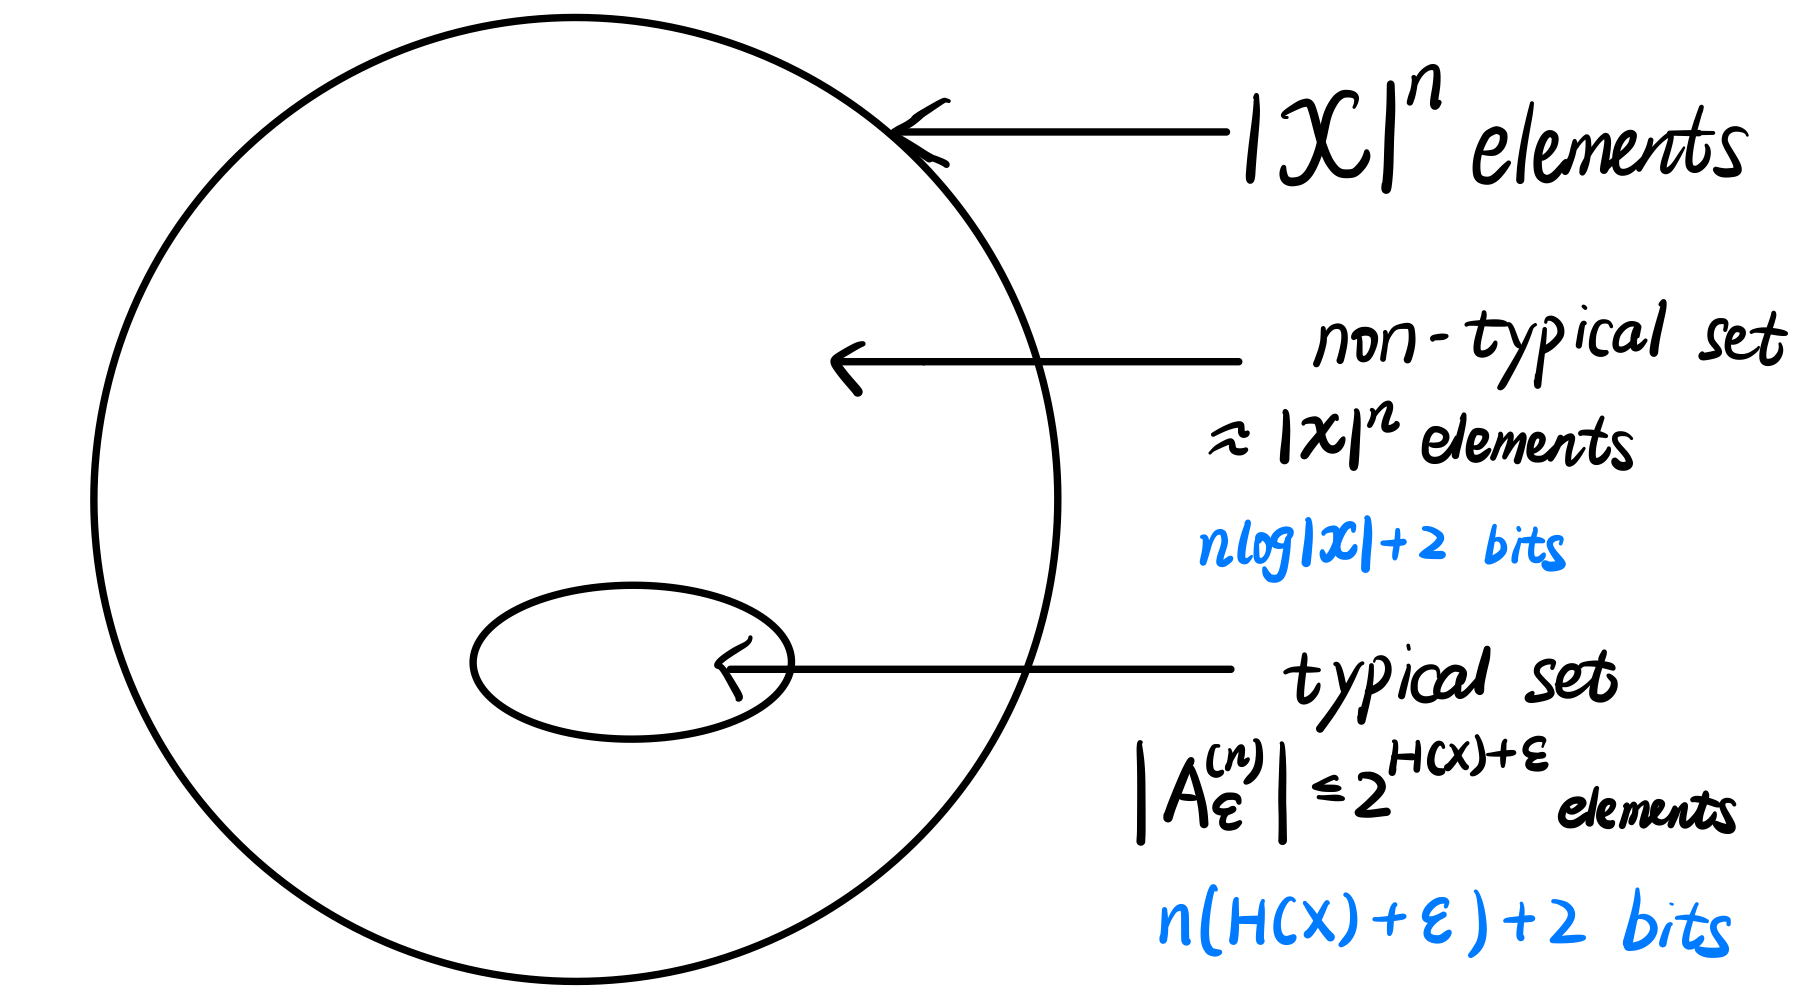
\includegraphics[width=0.8\textwidth]{./figures/chapter4/typical_set.png}
\end{figure}

\textcolor{red}{这说明$A_{\epsilon}^{n}$中的序列总数量较少(占所有序列的比例趋近于0),但是整体出现的概率都很高(任取一个序列时typical sequence的概率趋近于1)}

方案1: 只对typical set中的序列进行定长码编码, 不对 non-typical set中的元素进行编码. 这样的编码方式时有损的, 但是当$n\to+\infty$时, 信息损失趋近于0(遇到non-typical sequence的概率为0).

定长码的码长为 $L=\left\lceil\log\left|A_{\epsilon}^{(n)}\right|\right\rceil \to nH(X)+1$.
此时平均码长为
$$\overline{L}=\dfrac{nH(X)+1}{n}=H(X)+\dfrac{1}{n}\stackrel{n\to+\infty}{\to}H(X)$$


\textbf{方案2: Asympototically Optimal coding 渐进最优的编码方式:}

将typical set 和 non-typical set 分别用\textcolor{red}{不同长度的定长码}的方式进行编码

typical set中每个序列的编码长度:
$$L_n = \left\lceil\log\left|A_{\epsilon}^{(n)}\right|\right\rceil \leq \left\lceil n(H(X)+\epsilon)\right\rceil<n(H(X)+\epsilon)+1\textcolor{red}{+1}$$
Non-typical set 中每个序列的编码长度:
$$L_n^{(c)}=\left\lceil\log |\mathcal{X}|^n\right\rceil < n\log|\mathcal{X}| +1 \textcolor{red}{+1}$$
其中$\textcolor{red}{+1}$是用于区分此序列是typical set还是non-typical set.
$$\overline{L}=\dfrac{\left(1-\epsilon\right)\left(\left(H(X)+\epsilon\right)+2\right)+\epsilon\left(n
\log|\mathcal{X}|+2\right)}{n}\to H(X)$$
As $n\to+\infty,\epsilon\to 0$. 其中上面出现$(1-\epsilon)$的原因是typical set出现的概率是$p(A_{\epsilon}^{(n)})>1-\epsilon$.

这些编码方式都是渐进最优 Asympototically Optimal $\neq$ optimal的(optimal的还是Huffman coding). 当$n\to+\infty$时, 只是在理论分析上渐进最优, 但空间爆炸, encode, decode 费时, 所以实际不会使用.